\chapter{Model framework \label{chapter:modelfw}}

\section{Introduction \label{sec:frameworkintro}}


This chapter has two aims:

\begin{itemize}
	\item Explain the logical structure of the model framework used in thesis and how it is presented in the results chapters;
	\item Cover in more depth some of the specific issues arising from the logical journey of model development (section \ref{sec:nutsnbolts}).
\end{itemize}

The model framework uses the economic and spatial ideas from chapter \ref{chapter:location} and provides a structure for agents using them to interact. It is built using object-oriented programming, as discussed in section \ref{sec:abmiswhat}. Table \ref{tab:keytable} gives a key for the diagrams used to describe the logic of the model; these diagrams use the code relations between objects to do this. (Appendix \ref{apx:modelcodeoverview} describes the code more traditionally, using UML, and explains the code in more detail.) The rationale for this approach is to present the object structure and the logic of the algorithms in one diagram as clearly as possible, but they should be used in conjunction with the text description. As mentioned in the introduction, an \gls{oop} coding norm used here is to capitalise objects, when they are being discussed as objects. For instance, `Good' is a particular object, distinct from goods generally. 



\subsection{Chapter overview}

The chapter covers the following topics:

\begin{itemize}
%including an outline of how results from the model framework are presented in the results (section \ref{sec:elementsmodelframework});
	\item An overview of the model framework;	
\item How the theorisation of space costs in section \ref{sec:elementsmodelframework} is implemented in the framework (section \ref{sec:spacecostgoods});
	\item The (non-Agent) structural elements of the framework are explained (section \ref{sec:elementsmodelframework});
	\item The functioning of the agents themselves is then described (section \ref{sec:actorSetup});
	\item The `framework discussion' section picks up some essential elements of the model framework that make more sense to explain after the details of the framework itself have been laid out. These include key ideas on the way information is theorised and how \gls{eos} is structured (section \ref{sec:nutsnbolts}).
\end{itemize}

\section{Framework overview \label{sec:elementsmodelframework}}

This section gives an overview of the framework and what variables it uses. To start with, the following types of space are used in different model set-ups:

\begin{itemize}	
\item Spaceless (a dimensionless point); 
\item A two-region space consisting of two discrete points separated by a defined distance; 
\item A continuous, one-dimensional line (referred to as $R^1$);
\item A continuous, two-dimensional plane (referred to as $R^2$)		 
\end{itemize}

From the point of view of the thesis models, the differences between them boils down to how agents' location choices are restricted. All other model features remain the same. (This also means that discrete spaces can be `simulated' by simply restricting agents to binary location choices.) Agents make their distance calculations based on Euclidean distance from other agents' locations. 

The size of both $R^1$ and $R^2$ is kept to a value of $1$ in all models except those using the density cost in section \ref{sec:results}, where it is set to $2$ to allow People a more variable space to disperse into. In $R^2$, width and height are always kept the same. Some very basic differences exist between $R^1$ and $R^2$ when costs are changed. Most simply, whereas in $R^1$, a doubling of distance leads to a doubling of space covered, in $R^2$, the area covered is quadrupled ($\pi(2r)^2$ is $\pi 4r^2$). If, for example, potential economic agents are evenly spread across space, there is thus a four-fold difference in the number of new interactions the doubling enables.

This space is used by two types of agent: People and Firms. The key list of features used by each of these is as follows:

\begin{itemize}
	\item \textbf{People:}
		\begin{itemize}
			\item Location within one of the space types;
			\item Time to spend: one `day' per model iteration. For the models in chapter \ref{chapter:models}, People optimise this one day on distance (`commuting') and giving labour to employers in exchange for a wage. Or to frame it another way (see section \ref{sec:reframingpeoplecost} below), People `pay for' their wage and their commute cost with this one day. For the transmission belt model in chapter \ref{chapter:connectedModels}, People's one unit of time is exchanged directly for goods (which can include the distance cost for goods);
			\item A `\gls{lov}' / \gls{ces} utility function as described in section \ref{sec:CESbasics} with $\rho$ controlling their preference for a mix of goods;
			\item A density cost; the background for this was given in section \ref{sec:extsinspace} and section \ref{sec:densitycostsetupFramework} below outlines its application in the model framework. This is used in the models in section \ref{sec:results} and the final model set-up in section \ref{sec:tbmplusdensity}. Otherwise, it is set to zero, thus effectively `turned off'.
		\end{itemize}
	\item \textbf{Firms:}
		\begin{itemize}
			\item Location within one of the spacetypes;
			\item A wage they offer to People in exchange for their time; is fixed to $1$ unless otherwise stated. If a Person incurs a `commute cost', the time it takes them to commute is accounted for in the wage they get (see below for how this is formulated). As mentioned, the transmission belt model functions differently: People buy goods directly with time. The goods are thus their direct wage (see section \ref{sec:prodtowelfare} for the full explanation of this mechanism);
\item A price for the good they sell, not accounting for distance; so if a Person was at $0$ distance from a Firm, this is what they would pay. These are set to $1$ unless otherwise stated; the distance cost for moving this good is identical for all Firms in any given model run, unless otherwise stated;
\item A production function, used in the transmission belt models, that turns People's input into a single-good output quantity using the smooth \gls{eos} function given in section \ref{sec:prodfuncts};
\item A level of stock, again used in the transmission belt models.
		\end{itemize}
\end{itemize}

The `partial' models in chapter \ref{chapter:models} keep most variables fixed, selecting only specific ones to vary, depending on the analysis. The details of these are given in the relevant results sections. For the more `general' model in chapter \ref{chapter:connectedModels} agents have fixed locations (except for two cases, for reasons explained in that chapter). The main variable for the transmission belt models is good price: Firms are able to change this in order to target a stock level. In the transmission belt models, People buy goods directly with time, so there is only one distance cost to be incurred. Again, unless otherwise stated, all other parameters are fixed to $1$.

The rest of this chapter deals with the specifics of how these agent features are implemented in the thesis model framework. The next section explains the implementation of space costs, how they enter into the wage and good costs and how these can be reframed in order to create the idea of one spatial and one non-spatial cost. This idea is then used in the final transmission belt model in chapter \ref{chapter:connectedModels}.

\section{Implementation of space costs \label{sec:spacecostgoods}}

%Section \ref{sec:factors1} introduced the idea of factors and how they are used in the model. `Time as a factor' can only be used to do two things: `buy' movement or pay for other factors (either goods or money, which is then used to buy goods). Decisions using `time as a factor' happen in one model iteration, not over several as would be the case with many real-world time-based economic activities. If there is an intermediary stage of acquiring a wage, it still needs to be bought with time (or `labour'; these terms are synonymous for the thesis model). 

\subsection{Cost of moving goods \label{sec:costmovinggoodsFramework}}

A simple mathemathical way to describe the cost of moving goods across space is as follows. Let $P_g$ be the full cost of one unit of good $g$, $p_g$ the base per unit cost, before any space-costs; $c$ the cost to move one unit of this good over one unit of space, and $d$ the distance moved. Then - 

\begin{equation}
P_g = p_g + (c\cdot d)
\label{eq:spacecost}
\end{equation}

On a given model iteration, this will be the cost faced by agents wanting to buy the goods. In line with the simple approach to time, no distance will be too large for goods to travel during one iteration, but the total cost, including $cd$, may be too high. $c$ represents a catch-all variable for the generic costs of moving goods, whether due to weight, bulk or some other factor. In equation \eqref{eq:spacecost}, the addition or subtraction of weight would be reflected in $c$, and changes in value in $p$. This is also where `value density' (see section \ref{sec:costmovinggoods}) can be defined. The ratio of product value to physical size/weight bcomes $p/c$, with $c$ standing in as a proxy for generic per-unit shipping cost. 
%(It could also be defined to include other factors that produce \gls{increts} to distance; that is, the further a unit is moved, the cheaper per unit of distance it becomes, as variable delivery costs increase relative to fixed delivery costs.) 
%For the purpose of this section, the important point is to note the impact of varying $p_g$, $c$ and $d$. 
\subsection{Cost of moving people \label{sec:peoplemovingFramework}}

There is a hard limit to people's time: a flow of `one day per day' must be spent. Because of this, one way to model distance for People in the model is to build up from the idea of one `day' and the distance People can get in that day. This approach is as follows: 

\begin{itemize}
%\item For each model day, each agent is given $t=1$ to spend: in other words, they have `one day per day' and will aim to make optimum use of it. (See note below for more on this.)
\item For a given distance $d$, the time is takes to cover it is $t_{d}$. So, generically, $t_{d}=f(d,tech)$, where $tech$ is some technology that has an impact on the time taken. For many of the models, time to cover a given distance will be a function of the distance alone. However, the generic factor $tech$ here indicates that the amount of time to cover a distance may change. This is used as a way to consider the impact of varying the cost of commuting.
\item $tech$'s role in this function is separate from its cost. For example, if $t_{d}=d/tech$, the time taken to travel $d$ goes down as the level of $tech$ increases. It says nothing about $tech$'s cost. From the point of view of agents in the thesis framework, this cost is ignored: they pay only for the distance cost itself, not any further transport overheads. Relatedly, in the thesis model, agents do \emph{not} need to `buy' migration. That is, if an agent moves their permanent location, this is free. It costs them to move goods or move themselves to a workplace.
\end{itemize}

%Section \ref{sec:factors1} introduced the idea of factors and how they are used in the model. The approach to time as a factor is quite specific and needs some explanation. `Time as a factor' can only be used to do two things: `buy' movement or pay for other factors (either output or money). Decisions using `time as a factor' happen in one model iteration, not over several as would be the case with many real-world time-based economic activities. 
\subsection{The cost of moving people as a parallel to moving goods \label{sec:reframingpeoplecost}}

Section \ref{sec:wageselect} outlines in detail one approach to how People's time can determine their wage. Simply, the amount of time remaining to contribute to an employer will be less if a Person is further away. If an employer pays a given wage for a unit of time contributed, at $d=0$, the Person gets a full unit of wage. At the one day limit, however, they will get no wage at all. (This is, of course, another unrealistic approach: see below for further discussion on this.) The model can be set up so that People select employers on this basis. However, as section \ref{sec:spatialvsnon} will later explain, it is useful to understand the parallel between good movement and People movement when it comes to describing their effect on spatial outcomes. 

In the situation just described, if a Firm was paying a wage of $w=1$ and $tech=1$, the Person's wage will just be $w=t-d$, with the imposed condition that if $d$ is over the hard time limit, the Person cannot consider that Firm as an employer. This is easy enough to code but not a very satisfactory analytic approach. It also masks the difference between the non-spatial and spatial elements by subsuming them in one function.

It can be reframed in a way that parallels the description of good costs used in section \ref{sec:costmovinggoods} above. To do this, the cost element needs to be separated from the budget element, as follows. A Firm is not offering a wage: rather, they are selling a factor – in this case, money - in precisely the same way they sell goods at a given price. (This will also come in useful later when agents are exchanging factors other than money.) The amount supplied is just $g=f/p_g$, where $g$ is the supplied factor, $f$ is the payment and $p_g$ the price of $g$. 

In these terms, People are just buying money with time. The price a Firm will charge is as just stated: $p_g$ for one unit of money. What about the space cost element? The uniqueness of moving People, it has been claimed, is the hard limit to time, beyond which no wage can be bought. The good-cost function above would not do this job: regardless of how high the price goes, some small quantity is always demanded. The only way such a hard limit could work is if the cost of money becomes infinite at the hard limit. This can be done as follows, using the variable definitions already given above. At the point where $d/tech = 1$, $p_g$ is divided by zero and the cost becomes infinite:

\begin{equation}
P_g = \frac{p_g}{1 – (d/tech)}\label{eq:wagespacecost}
\end{equation}

A Person with a time-budget of $t=1$ must optimise given these costs. Assuming they are only `buying money' from one Firm (an assumption changed later) , they will want to spend their whole budget on the single cheapest supply. The amount they can buy in this situation is just their budget divided by the full price described in \eqref{eq:wagespacecost}. Assume $t$ and $tech$ equal one, then the amount they can buy is just their time divided by the price:

\begin{equation}
g = \frac{t}{p_g/(1-d)}\ = \frac{(1-d)t}{p_g}
\end{equation}

This brings the description full circle: if the `price of money' is one, the amount the Person gets is proportional to what is left after distance has been accounted for. 

What was the point of this long roundabout trip? Three things: firstly, to highlight that the more algorithmic description of People getting their wage can be reframed into a simple optimisation problem with a price and a budget. Secondly, to illustrate that different cost functions can be made to achieve particular spatial outcomes. Thirdly, it helps in reframing all movement costs as one combined cost in chapter \ref{chapter:connectedModels}, where People are paid directly in goods using the less hard-cutoff cost equation \eqref{eq:spacecost} above.
%Lastly, as mentioned, this allows the clear separation of the `cost of money' and the space cost involved, which here is controlled by $tech$. Section \ref{sec:spatialeq} will use this to compare the effects of spatial versus non-spatial cost change. 

\section{Density cost \label{sec:densitycostsetupFramework}}

As section \ref{sec:extsinspace} explained, the model framework uses a density cost as a proxy for both land costs and generic congestion, covering all `costs of proximity'. The density cost is imposed on agents in proportion to the number and proximity of others within a set radius from that agent's current location. This section outlines how the density cost is calculated and applied as well as providing a rationale for this approach. This use of density cost is very simple, but would be prohibitively difficult in anything but an \gls{abm} setting. It requires each agent to make their calculation individually while taking account of others' location. 

The density cost uses three parameters. First, a radius around each Person within which density costs are incurred. Second, a variable capturing the density of People within that radius, returning a normalised value between zero and one. The resulting value would be one if all agents are on exactly the same spot as `me' (this never happens in practice; see below), zero if none are within the density cost radius, and between zero and one otherwise. It is worked out for each Person as follows:

\begin{itemize}
\item Using the density cost radius, normalise each other Person's distance from `me' to between one and zero, where one is the same location as `me', and zero is on or beyond the radius.
\item Sum these normalised distances, then divide by the total number of People in the model run.
\item Thirdly, this normalised density cost variable is then multiplied by a factor that determines its overall effect. 
\end{itemize}

This final density cost value is imposed directly by subtracting it from People's wage. Note that the density cost is independent of the wage, so it becomes proportionately smaller if wages are higher. 

%The values used for the density cost parameters are important only insofar as how they interact with other key variables like wage and distance costs. 
The radius is kept to $1/32$ of the width of model space, which itself is normalised to $1$. The radius is arbitrary, as it can be calibrated to agent number and density cost to produce the morphological outcomes: it is chosen to allow a clear graphical view of outcomes. For most density-cost-based models (section \ref{sec:results})  the multiplication factor is set to $10$ as this allows a range of spatial outcomes where People can find trade-offs between density cost and distance. By increasing the multiplication factor, section \ref{sec:notutilityeq} shows what happens when agents are pushed outside of this trade-off range: utility equilibria start breaking down.

%Save any other spatial costs, a density cost by itself is, naturally, dispersive. The point of economic interest is how agents choose to trade that cost off against other benefits they find from choosing a particular location: models examining this result are presented in section \ref{sec:results}. 
%CEUS Repeats
%The fact that the density cost is centred on a mobile agent is counter-intuitive: surely land is an immobile factor? However, on a featureless plain where no exogenous difference in land quality is imposed, its cost must be considered as part of the other costs and benefits of being on that spot. From this point of view, a farm has the same considerations as a factory or a house: how much land is required to produce a given output, and how does its location affect proximity to other important economic agents? 
%The trade-off agents in this paper must make is similar, based on `second nature' relative location effects (in contrast to `first nature' geographical features with absolute location). Second nature effects thus come about through interaction between locations. Though O'Sullivan and Unwin point out, ``it is usually impossible to distinguish these effects in practice simply by observing the intensity of a process as it varies across space'' (\citealt{osullivan_geographic_2002}, p.79), providing agents with a density cost is inherently `second nature'. In the models presented, only Firms are `first nature', having a fixed location.
%The density cost is the medium of interaction between agents. Without it, each would make decisions entirely independently of the others, with no actual difference between running a model with one agent a hundred times, or a hundred agents once (i.e. it would be ergodic). Using density cost as a proxy makes the connection between land and distance costs vital to monocentric models. Density cost supplies the same thing that Alonso required consumption of land quantity for\footnote{``If the only criteria for residential location are accessibility to the centre and the minimising of the costs of friction, and considerations of the size of the site are excluded, all residence would be clustered around the centre of the city at a very high density.'' \citealt{alonso_location_1964} p.9}: an economic reason for distance to exist at all in a model trying to explain spatial morphology ``as an endogenous outcome of the economic process'' (\citealt{storper_agglomeration_2010}, p.315). The density cost avoids a `black hole' outcome: agents do away with space altogether if they can, collapsing into a single point (\citealt{fujita_location_1999} p.58).

\section{Elements of the model \label{sec:elementsmodelFramework}}

\subsection{Key table \label{sec:keytable}}

Table \ref{tab:keytable} lists a series of graphical components used in figures below to help illustrate how the model framework is put together and how it functions.

%%%%%%%%%%%%%%%%%
% Key table
%%%%%%%%%%%%%%%%%
%http://texblog.net/help/latex/ltx-68.html
\renewcommand{\arraystretch}{1.2}
\begin{table}[!hbt]
\begin{center}

%\begin{tabular*}{0.8\textwidth}{|l|l|}
\begin{tabular}{|l|l|}
\hline 
\textbf{Element} & \textbf{Description}\\
\hline
\raisebox{-3mm}{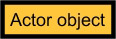
\includegraphics[height=6mm]{ChapterFramework/figures/keybits/actorobj.jpg}} & People or firms\\
\hline
\raisebox{-3mm}{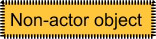
\includegraphics[height=6mm]{ChapterFramework/figures/keybits/nonactorobj.jpg}} & Any other object used in the framework\\
\hline
\raisebox{-3mm}{
\includegraphics[height=6mm]{ChapterFramework/figures/keybits/variable.jpg}} & Grey boxes indicate variables.\\
%\raisebox{-3mm}{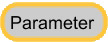
\includegraphics[height=6mm]{ChapterFramework/figures/keybits/parameter.jpg}} & Parameters are fixed for model runs but may change between them\\
%\raisebox{-3mm}{
\includegraphics[height=6mm]{ChapterFramework/figures/keybits/constant.jpg}} & Constants do not change\\
\hline
\raisebox{-3mm}{
\includegraphics[height=6mm]{ChapterFramework/figures/keybits/objarray.jpg}} & An array, or set, of objects, such as the set of all firms\\
\hline
\raisebox{-3mm}{
\includegraphics[height=6mm]{ChapterFramework/figures/keybits/ref2obj.jpg}} & For example, a Person may want to keep a reference to their preferred employer\\
\hline
\raisebox{-3mm}{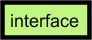
\includegraphics[height=6mm]{ChapterFramework/figures/keybits/interface.jpg}} & A way to provide shared methods to different objects; not important for\\
&understanding model logic, but worth noting where present\\
\hline
\raisebox{-3mm}{
\includegraphics[height=6mm]{ChapterFramework/figures/keybits/method.jpg}} & An object method for achieving a particular model aim\\
\hline
\raisebox{-3mm}{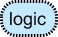
\includegraphics[height=6mm]{ChapterFramework/figures/keybits/logic.jpg}} & Can be one of three things: a logical decision, a calculation\\
& Or an operation on a set (array)\\
\hline

\end{tabular}

\caption{Key for model diagrams \label{tab:keytable}}
\end{center}
\end{table}

\subsection{Decision structures and model timeline \label{sec:frameworkDecisionStructures}}

\begin{figure}[h!]
\centering
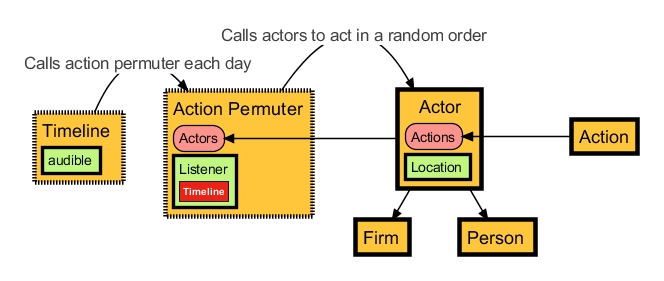
\includegraphics[width=0.75\columnwidth]{ChapterFramework/figures/TimelineActions}
\caption{Timeline sequence \label{fig:frameworkTimeline}}
\end{figure}

The timing structure shown in figure \ref{fig:frameworkTimeline} is very simple: as each day passes on the `Timeline', an `Action Permuter' calls Actors in a given order.\footnote{The Timeline is part of an Observer framework used by other model elements like visualisation and data writing; again, see the code appendix for more details.} The issues around exact ordering are discussed in section \ref{sec:randomisation}. When an Actor is called, they decide what action to take. Actors' decisions can use any of the following:

\begin{itemize}
	\item Instant: act on information collected `now'
	\item Feedback: Act, wait, respond
\end{itemize}

As discussed in section \ref{sec:blindvsrational}, agents take decisions either instantaneously or using feedback from their actions over one or more timesteps. In instant decisions, when agents are called to act, they immediately gather the information they need and optimise based on that. For multi-timestep decisions, agents try an action and then check later whether the outcome was desirable or not before taking their next action. No attempt is made to simulate synchronous decision-making. At the point where an agent is deciding, all others are currently static.

Outside of the Timeline-driven decision structure, there is a third type of `reflex' decision that Actors can take. Here, an Actor is coded to react to requests from other Actors, rather than the Timeline - for instance when a purchase takes place. These reflex actions are mostly just the exchange of stock or money, but can also involve adjusting prices in a `granular' way, rather than the Actor waiting for their decision turn. For instance, this is used in the model in section \ref{sec:prodtowelfare} where granular price-changes are used to equilibriate stock levels.

\subsection{Two agent data sources}

Actor decisions will be based on one or both of the following sources of information:

\begin{itemize}
	\item Internal Actor data, changed by other agents since last a decision was taken. (Example: Firm net income.)
	\item Externally collected data (Example: list of good prices from surrounding Firms.)
\end{itemize}

Externally collected data can come only from other Actors. This is acquired by searching for a list of all appropriate Actors and forming a set from it.

These three elements - Actor setup, decision structure and Actor data - form the foundation for the model framework. Because all agents face a static world at the point where they decide, their actions can be logically described separately: section \ref{sec:actorSetup} explains how they are put together. 

\section{Agent setup \label{sec:actorSetup}}

\subsection{How People act \label{sec:howPeopleAct}}

\begin{figure}[h!]%
\centering
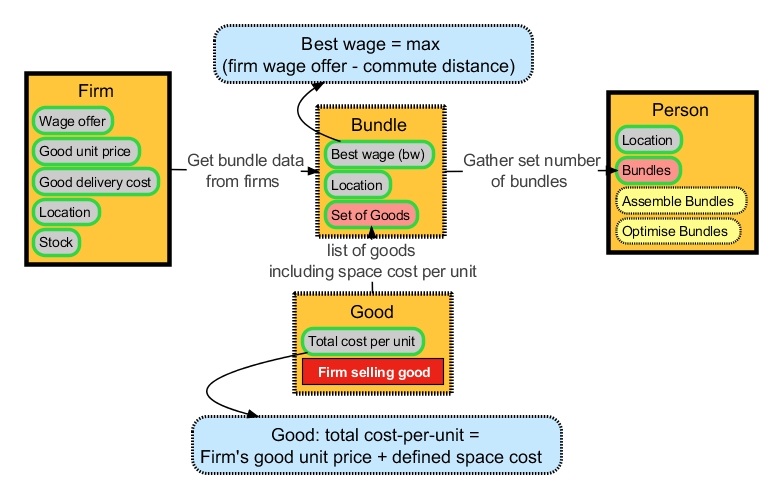
\includegraphics[width=0.95\columnwidth]{ChapterFramework/figures/PersonAction1}%
%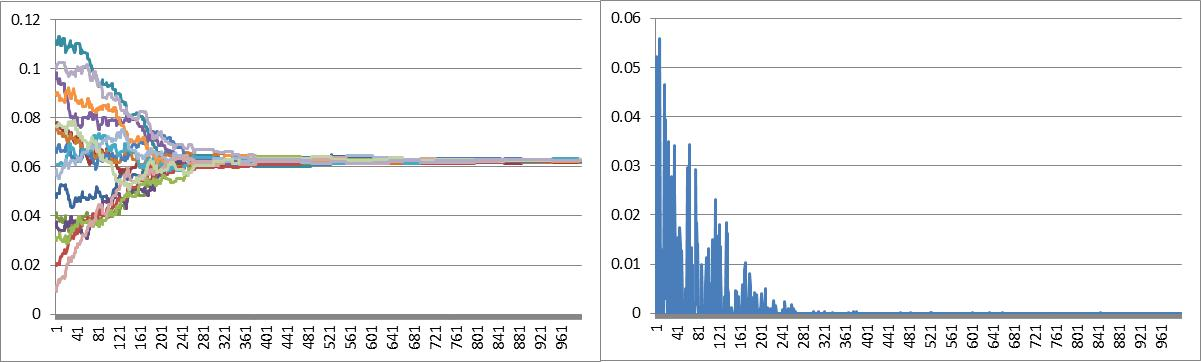
\includegraphics[width=0.85\columnwidth]{ChapterTestingModels/Figures/hillclimbExcel}%
\caption{Elements for the Person action}%
\label{fig:personlogic1}%
\end{figure}

%\subsection{How do People turn time into utility? \label{sec:turntimetoutil}}
People have `one day per day' to spend and their fundamental question is, `what is the maximum utility I can get for my time?' This time can be spent on moving through space or put into Firms in exchange for either goods or money. The description here deals with the most complex of these: People working for money and then spending it on goods. 

\subsubsection{Bundles: overview \label{sec:bundles}}

The Bundle is central to the way People optimise their utility, tying the previous framework sections together. When it is each Person's turn to act, they look to find better economic options in different locations. They do not attempt to exhaustively search all of model space. Instead, they assemble a set number of `Bundles', each centred at randomly chosen points. They also include a Bundle for their current location to check whether staying put is the best option.

Each of these Bundles contains all the economic information needed to calculate a utility level for that location: the cost of all available goods, including delivery cost; the cost of accessing a wage, including the commute; and the density cost that would be incurred if residing there. Once utility is worked out for each of these Bundles, the best is selected and, if this is not on the current spot, the Person moves there.
%They contain spatial as well as economic information: each is centred at a given coordinate in model space and records locations of potential employers and good suppliers relative to that.

Figure \ref{fig:bundleViz} illustrates this process for the first two iterations of a model run. The particular set-up is that from results section \ref{sec:results} as this includes the density cost and provides a clear view of where the agents are located. To help illustrate the Bundle process, ten Firms (indicated with crosses) are located randomly and People use a `love of variety' utility function, buying a mix of goods (see section \ref{sec:LoVresult} for more details on this function). The figures pick out a typical Person (marked as a triangle). That Person's range of Bundle sample points are shown, with small, black squares being lowest utility value and large, white squares the highest. A thick black circle marks the best utility Bundle; lines indicate where that best Bundle will acquire goods, with thickness of lines in proportion to budget spend on each. Sub-figure \ref{fig:bundle1} shows a Person's initial best Bundle; sub-figure \ref{fig:bundle2} illustrates their move to this Bundle and sampling again to find the next. The process of assembling Bundles is as follows:

\begin{itemize}
\item Create a set number of empty Bundles, each with randomised centroid coordinates in model space. 
\item For each Bundle, relative to its centre, work out:
\begin{enumerate}
\item What is the optimum wage the Person could get from that location? (What is the most money they can buy with their time, accounting for the base wage, commute distance and density cost?)
\item What is the optimum utility the Person could get, given the optimum wage, the total price of goods (accounting for distance) and their utility function?
\end{enumerate}
\item Select the bundle with the best utility: move to that location, take wage and buy goods. (Note: People do \emph{not} need to `buy' this movement between points. That is, when moving location, this is free. It costs only to move goods or move themselves to a workplace.)
\end{itemize}

As mentioned, each Bundle's found utility level is `objectively' true at the moment it is calculated. However, a Person's set of Bundles is only a very small random sampling of the space around them: a subset of random locations within a given small radius of the Person's current location and another set randomly chosen from the whole space. This allows a balance between finding small extra incremental benefits nearby with having a good chance of finding better options wherever they may be. However, it is almost certain that a small sample of locations will not find the objectively best spot in one iteration. For the method to be successful, this sampling procedure needs to be repeated over many timesteps until no Person is able to unilaterally improve their utility level (a Nash equilibrium). The Bundle sampling process does converge on a stable outcome: People gradually cease moving location as all available options for better utility are exhausted.

\begin{figure}[p]
\centering
\subfloat[time t]{\label{fig:bundle1}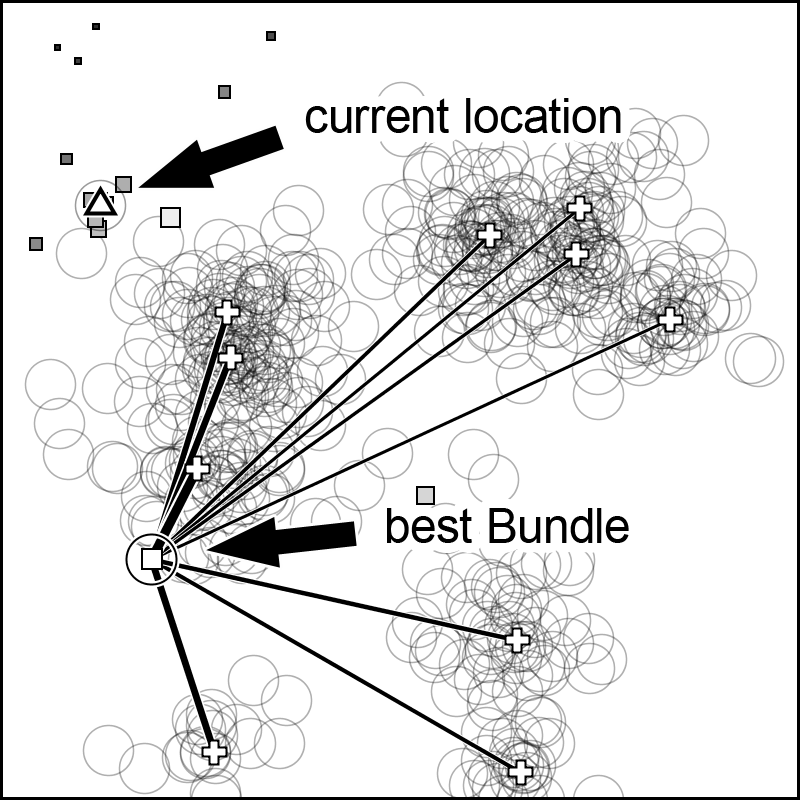
\includegraphics[width=0.6\textwidth]{ChapterFramework/figures/Bundle1border}}%
\hspace{0.1} 
\subfloat[time t+1]{\label{fig:bundle2}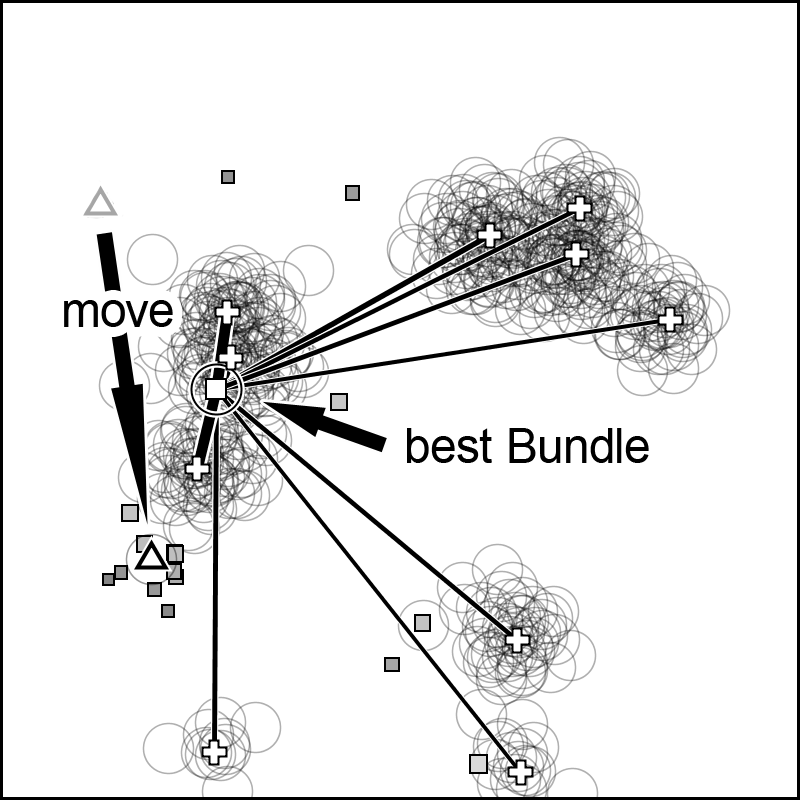
\includegraphics[width=0.6\textwidth]{ChapterFramework/figures/Bundle2border}}%
\caption{Bundle sampling and selection for two iterations, focusing on one Person (white triangle). Other People's density cost radii indicated in light circles. At time $t$, the Person finds a `best Bundle' having compared a set of Bundles including density cost and good prices through a CES function. \label{fig:bundleViz}}%
\end{figure}

\subsubsection{Selecting the best wage \label{sec:wageselect}}

The `transmission belt' model in chapter \ref{chapter:connectedModels} allows People to spent their time on a range of Firms through a \gls{ces} function. This provides a way to avoid \gls{bertcomp}: People choosing whichever employer is the cheapest, thus usually the nearest. Section \ref{sec:examplesmapping} discusses this point further. The rest of this section outlines how, in the rest of the model runs, People choose a Firm to give their time to. 
%How does the Person decide who to contribute to? The simplest method allows them to know exactly which option will give them the highest utility and select accordingly. This is not always directly possible, for reasons discussed below. The next simplest is to use price: they choose the highest price on offer for their input, or using a function like the \gls{ces}, they can buy a utility-maximising mix of available outputs. Section \ref{sec:prodtowelfare} presents a model of this type, where the more challenging problem of using price to signal between production and welfare is discussed. 

Each Bundle has one unique `best wage' offer. Selecting this is a two-step process: first, gather a set of all Firms within commute distance. Second, select the Firm offering the best wage, accounting for commute distance from the Bundle's location centre. This best wage can be described as follows. Let $F=\{f_{1},f_{2},...,f_{n}\}$ be the set of Firm objects. Each Firm has a wage offer, which is `the amount paid for one day's input'. For each $f\in F$, $W_{f}$ is that wage offer. To describe space cost, the distance in \emph{time} can be used: for each $f\in F$, $t_{fa}$ is the time taken to travel between $f$ and $a$. 

Let $l_{af}$ be the labour available to contribute to $f$ by Person $a$. The amount of labour they have available for contributing is just their own time (one day, $t_{a}=1$) minus commute time. Here, a `commute' is taken to be twice $t_{af}$. The upper distance limit on whether a Firm enters into $a$'s considerations has to be less than $a$'s one available day in total - half a day there, half back - otherwise there is no time left at all to contribute to production. So $f$ can only be a maximum of half a day away. Given all this -

\[
l_{af}=t_{a}-2\cdot t_{af},\; 0<l_{a}<1\]

If $W_f$ is $f$'s wage for a full day, and $a$ has $l_{af}$ to contribute (a fraction of their full day), this means the wage they will get is just $W_{f}\cdot l_{af}$. The best wage for Person $p$ can now be defined as:

\begin{equation}
bw_p=max\; \{W_{f}\cdot l_{af}\mid W_{f}\in F,\; t_{af}<0.5\}\label{eq:bwpmax}
\end{equation}

So, the best wage for Person $a$ is the maximum value from the following set: all wage offers proportionate to Person $a$'s labour input from those Firms in $F$ who are less than half a day away.

\subsubsection{Optimising bundles \label{sec:optimisingbundles}}

\begin{figure}[]
\centering
\subfloat[16 initially randomised good costs converge on utility-maximising value]{\label{fig:hillclimbgoodcost}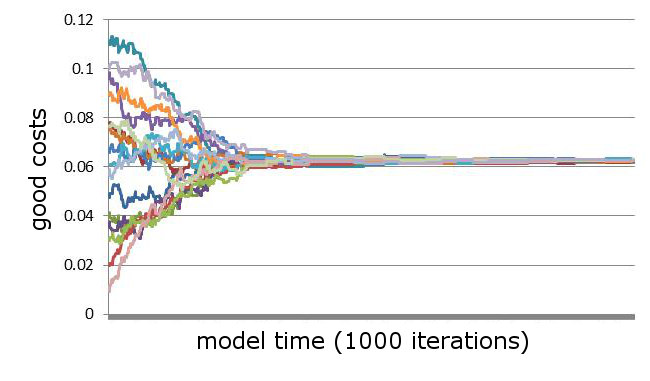
\includegraphics[width=0.78\textwidth]{ChapterFramework/figures/hillclimbExcelGoodCost}}%
\hspace{0.1} 
\subfloat[Marginal utility gain (change in utility between hill-climber iterations)]{\label{fig:hillclimbmarginalgain}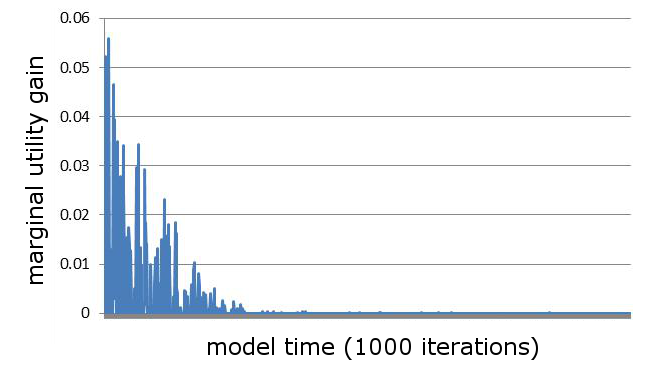
\includegraphics[width=0.78\textwidth]{ChapterFramework/figures/hillclimbExcelMarginal}}%
\caption{Utility-maximising hill-climbing algorithm, optimising a CES function with 16 goods over a thousand iterations, showing both randomised good costs converging on the utility-maximising level and the marginal utility gain for each step over 1000 iterations. \label{fig:CESHillClimbIllustration}}%
\end{figure}

Once a Bundle is assembled, it can be passed to the Person's optimisation routine.\footnote{As appendix \ref{apx:modelcodeoverview} explains, there is only one actual, static Optimiser class, but in terms of a `functional mapping'  it can be considered internal to each Person.} This produces a utility level from one of two possible utility-maximising methods, and the result is stored in the Bundle. Finally, the Bundle with the maximum utility level is selected: the wage offer is accepted and the optimal quantity of goods is bought.

The logical goal is simple: for each Bundle, find out how to spend the best wage on the set of Goods as optimally as possible (without actually spending it) then choose the optimal Bundle. Figure \ref{fig:personoptfr1} is an overview of the process. Assuming the Person has the set of Bundles they will optimise, the sequence is as follows. 

\begin{figure}[]
\centering
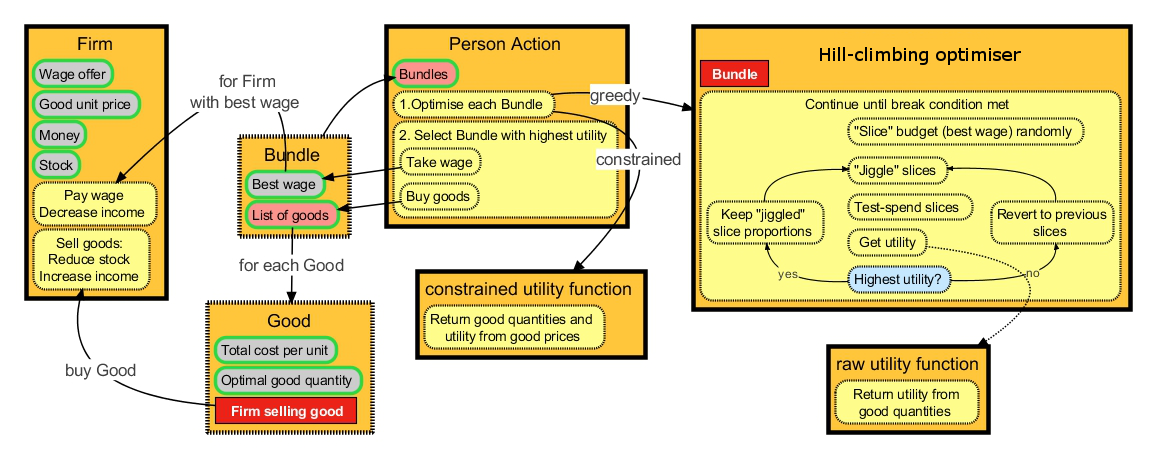
\includegraphics[width=1\columnwidth]{ChapterFramework/figures/PersonOpt2edit}%
%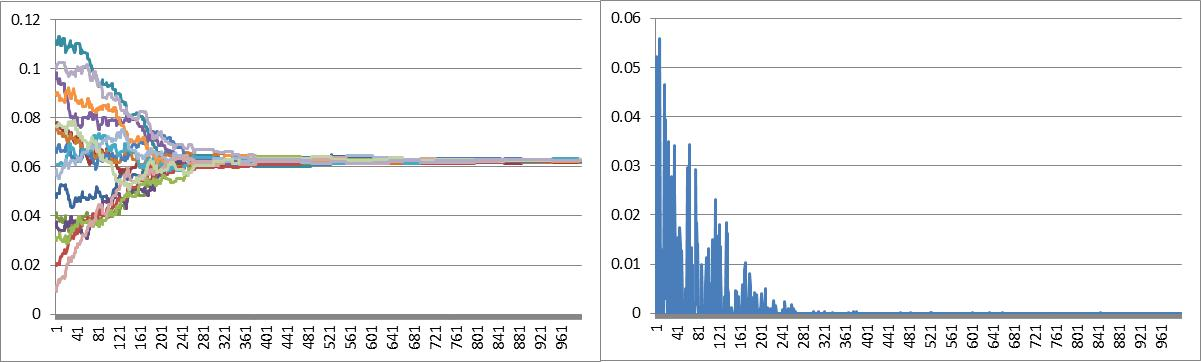
\includegraphics[width=0.85\columnwidth]{ChapterTestingModels/Figures/hillclimbExcel}%
\caption{Optimisation of Bundles in a Person's action}%
\label{fig:personoptfr1}%
\end{figure}

\begin{itemize}
	\item Optimise each Bundle. This happens in one of two ways:
	\begin{itemize}
	\item $(1)$ A `hill climber' optimiser uses the following method - 
\begin{itemize}
\item The hill climber iterates for a set number 
	\item The iteration is initialised by randomly slicing the budget (the best wage), one slice for each Good in the bundle, before beginning the iterations, so that each has a starting guess price. The iterations are:
	\item `Jiggle' the slices, changing their proportionate size slightly.
	\item `Test-spend' those slices on each Good: find out how much could be bought with the current budget slices using the per-unit price for the Good.
	\item Get a utility level for these quantities of goods. The Utility function is logically separate: the Optimiser deals only with this process of random slicing and adjusting.
	\item If the utility level found is the highest so far, keep the current proportion of slices and return to the 'jiggle' point. Else, revert to the previous slice proportions and try again. This has the effect of ratchetting the budget slices (and thus the spend per Good) towards an optimum.
\end{itemize}
	\item $(2)$ `Constrained' optimiser: a Bundle is passed directly to a code version of the constrained utility optima described in section \ref{sec:constrained}.
	\begin{itemize}
	\item{The Good prices and budget are used to directly calculate optimal good amounts. The utility level is then `read back' from those amounts.}
	\end{itemize}
	\end{itemize}
	\item Once each Bundle has an optimum utility, select the Bundle with the highest utility, then:
	\begin{itemize}
	\item Take the best wage: this instructs the Firm to pay the Person.
	\item Buy goods in the quantities found optimal by this Bundle.
	\end{itemize}
\end{itemize}

Figure \ref{fig:CESHillClimbIllustration} graphs data from the hill-climbing algorithm in action. A bundle containing sixteen goods of equal cost is optimised for a CES function over a thousand iterations. (The optimum for a CES function with equal-value goods is  already known from section \ref{sec:CESbasics}: an even mix.) In this example, the optimum is found quite slowly: this helps to illustrate the process. The first graph shows initially random budget split guesses converging on the optimum mix of $0.06$ for each good. The second shows the marginal utility gain from each iteration; most of the gains happen very quickly, after which almost no extra benefit accrues (though there is a very small amount of further convergence.)
%The important difference to analytic constrained optimisation is that people can work with any number and type of good and can deal with limited stock levels. If People find an optimal amount simply isn't available to them, they must spend their wage accordingly. 
%In contrast, a standard constrained optimisation results in an `objective' optimum (see \ref{sec:produtility_agents}). In this model framework, people may find that this optimal amount simply isn't available to them, so they must spend their wage accordingly. As well as being able to deal with any quantity of available good, this approach also allows easy swapping of utility 

%\begin{figure}[h!]
%\centering
%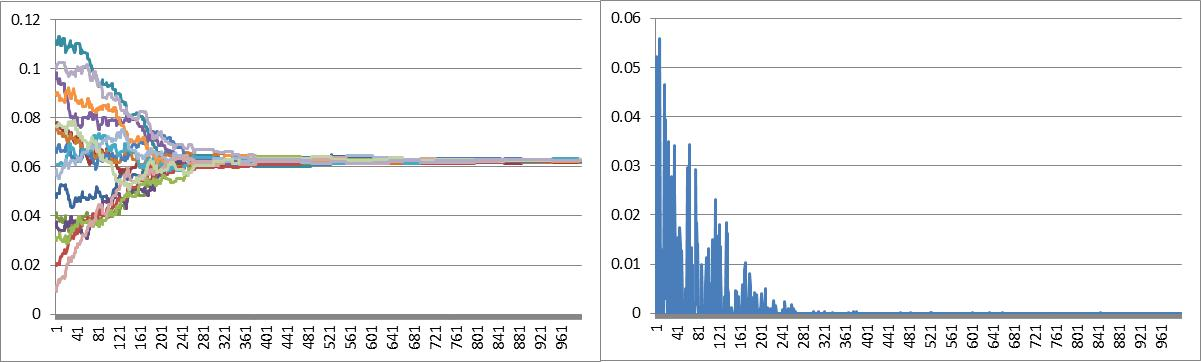
\includegraphics[width=0.85\columnwidth]{ChapterTestingModels/Figures/hillclimbExcel}%
%\caption{Utility-maximising stochastic search algorithm, optimising a CES function with 16 goods over a thousand iterations (x axis)}%
%\label{fig:CESHillClimbIllustration}%
%\end{figure}

\subsubsection{Overview of People's utility \label{sec:frameworkUtility}}

The technical detail of optimising utility has just been covered. There are three further points worth covering briefly.

People have utility functions based on those described in section \ref{sec:econconceptsintro}. In any one model run, all agents have identical tastes: they all use the same utility function. One useful assumption from using identical tastes is that, in one-good models, only the absolute quantity of that good matters. This is because the same quantity of good will always return the same utility for each Person, regardless of the form of utility. For example, if all People have an identical one-good utility function that happens to have \gls{increts}, the \gls{increts} will just produce the same level of utility for everyone, given the same good input. In contrast, if tastes were not identical, one Person could gain more utility from the same quantity of good as another. Many of the simplest model tests use the assumption that a single good quantity can stand in for utility.

In all situations where more than one good is available, People use utility functions. The form of utility used must also imply the production structure, though not the actual production function itself. For instance, a two-good utility function means a model where only two goods are made, though many Firms may compete to sell each good. An $n$-good utility scenario, using the \gls{ces} function, will have each Firm making one unique good, as they do in \gls{monocomp} models.

Actors using this method are rational in only the most basic way: they are able to judge when one Bundle is better than another. This rationality reflects basic micro-economic preference assumptions. Bundles of goods are `complete': any two bundles can be compared. They are also transitive: as Varian puts it, ``if the consumer thinks that $X$ is at least as good as $Y$ and that $Y$ is at least as good as Z, then the consumer thinks that X is at least as good as Z'' (\citealt{varian_intermediate_2006} p.35). 

%Things to do here:
%Give a run-down of the actual utility details and how it fits together
%Give a run-down of the structure of the optimisation
%Why take this approach, when it is possible to produce constrained optima that include price? 
%MM1 20pp/23	Reasoning behind bundle approach; cf. to Fowler's 'objective demand' approach. Write up.
%again, I'm not sure where to discuss the hill-climb, the black-box nature of it, compared to some `online' approach. At the moment, I haven't used the online approach, so I'll leave it. Needs discussing somewhere
\subsection{How Firms act \label{sec:howFirmsAct}}

In many of the partial models, Firms take no actions at all: they serve as geographical points of good supply only. Where they do take actions, there are two types. In chapter \ref{chapter:connectedModels} the decision process is `granular': it is explained in-depth in that chapter as it ties very closely to the explanation of the stock targeting mechanism used. 

All other Firm decisions come into the \gls{dmr} category (see section \ref{sec:dmr} for more details). The method used is as follows. A Firm's decision process is based on feedback between timesteps. A Firm takes an action, waits, and then responds depending on how its own internal data has changed (see figure \ref{fig:FirmAct1}). Because of this, the structure of Firm decision-making is quite a lot easier to describe, since Firms do not collect any data externally themselves. 

At time $t-1$, a Firm perturbs its current geographical position\footnote{The model framework explored perturbing location, good unit cost or wage offer; only location is considered here as the others faced problems. This is discussed in more detail in section \ref{sec:partialtogeneral}.}, altering it slightly in a random direction. It remembers these choices. At time $t$ the Firm asks, `did my net income between timesteps increase?' If yes, it repeats the previous action (hence needing to remember what it was), with the possible addition of increasing the size of the adjustment. If not, the Firm returns to its original location and re-initialises the random search.

\begin{figure}[]%
\centering
\includegraphics[width=0.85\columnwidth]{ChapterFramework/Figures/FirmAct1}%
\caption{A Firm's feedback mechanism: ``jiggle'' a random value, wait to see effect.}%
\label{fig:FirmAct1}%
\end{figure}

The result is that, through blind search, Firms are constantly searching for ways to improve their net income. Note that this method disconnects them even further from any analytic approach to optimising. Where People do use a utility function, the Firm does not directly consider its own input or output requirements. 
%Also, while they act on how their own internal data changes, Firms know nothing about how those changes occur. 

%\subsubsection{Firms' production functions}
%\cmt{This is all described in chapters 2 and 4. What do I want to say here? Something specific? It only counts for the one model so far. Uhmmm.}
%The simplest Firm production function turns a given amount of labour input into good output. For a given time period, how can this be worked out? Section \ref{sec:dmr} explored the problems of getting agents to utilise \gls{increts} in an agent-based time structure. The goal is to allow the model's Firms to gain from those \gls{increts}: output per unit of input labour should increase as the total labour contribution rises. The problem is finding an effective way to allow that total labour quantity to change, given the discrete, asynchronous nature of decision-making.
%The solution used is as follows. Two things happen: first, when a Person chooses an employer, they receive their wage on the spot, and their contribution to the Firm's production is calculated then and there. However, they `leave' a record of their contributed time with their chosen employer until it is their turn to act again, when they remove it and decide anew. This means that, when anyone else comes to contribute, that time is still considered as an input, as far as the production function is concerned. This allows \gls{increts} to occur. This approach is discussed in more depth in section \ref{sec:backyard} to see exactly what impact its assumptions have on model outcome.

\section{Framework discussion \label{sec:nutsnbolts}} 

\subsection{Interdependence of decision structures \label{sec:decstruct}}

It is not easy to meet the \gls{oop} ideal of fully encapsulated, autonomous agents in an economic modelling scenario. Indeed, it could be argued that in an economic modelling situation, it is not desirable. Much of the agent literature seems to have absorbed a modelling paradigm required for `instrumental' agents able to carry out real-world tasks. For example, Wooldridge's `Introduction to Multi-agent Systems' mentioned in chapter \ref{chapter:ABM} is imbued with this sense of the need for autonomous agents,  where ``each agent is assumed to have at least one thread of control'' (\citealt{wooldridge_introduction_2009}). 

Putting aside reasons of computational expense, programming fully autonomous economic agents in this way is a massive task. This becomes particularly apparent when trying to construct the timing framework. The ideal of fully independent objects mediating their interaction with a separately threaded environment is a stark contrast to the reality of the interdependence of different agent decisions. This section looks at a number of examples of this that arose during model development, and includes references to results in chapter \ref{chapter:models} that examine these problems more closely.

Any decision which will, in the process of optimising, interact with other agents' decisions can be considered `online'. In contrast, an agent able to optimise a utility function without affecting the basis for its optimisation is `offline'. The terminology is Holland's: Mitchell describes its use in the `two-armed bandit' game, where the player tries to discover each arm's mean payoff and variance:

\begin{quote}
``... the goal is not merely to guess which arm has a higher payoff rate, but to maximise payoff in the course of gaining information through samples to the two arms.'' (\citealt{mitchell_introduction_1998} p.119 discussing \citealt{holland_adaptation_1975})
\end{quote}

The difference between off- and online decision-making is partially blurred with many agents, and depends on timing structures. For the two main types of decision described in section \ref{sec:frameworkDecisionStructures}, `instant' is partly offline, since Actors face a static world and can select the objectively best Bundle. It is also partly online, in that the global optimum is affected by the number of random Bundle locations they can test at any one time; the movement towards a global optimum is thus not instantaneous, and Actor choices interact. This can lead to path-dependence for single Actors, but the global outcomes are statistically identical at the aggregate level. The `feedback' decision process actually relies on being `online' since the Actor requires the `world' to respond to its action to know what to try next. This is discussed in-depth in section \ref{sec:dmr}.

\begin{figure}[p]%
\centering
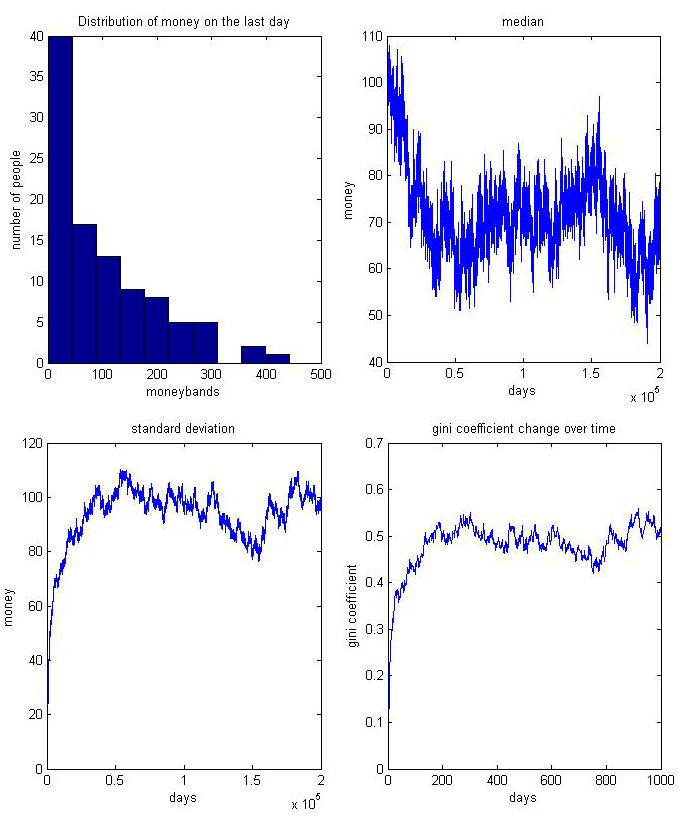
\includegraphics[width=0.98\columnwidth]{ChapterABM/figures/simplemoneytest2}%
\caption{Zero-intelligence agents exchange finite money, beginning with equal amounts. Top left figure shows the distribution of money on the last model day: a few very wealthy agents emerge while most are in the lowest $0-50$ band. \label{fig:simplemoneytest}}%
\end{figure}

\subsection{Communicating costs \label{sec:comm_costs}}


Agent models proceed over many iterations. In a spatial economic model involving goods, this presents two immediate problems that need solving. Firstly, in such a world, what moves between economic linkages each timestep: actual resources, where agents actually `exchange' some excludable, rivalrous quantity? A common way to avoid this is to presume goods perish before the next timestep (e.g. Tesfatsion's `hash and beans' model; {\citealt{tesfatsion_agent-based_2006} p.848). In the thesis model, where good stock is not fixed, the presumption of both persistent and perishable stock are tested to see the effect on the link between production and welfare (see section \ref{sec:prodtowelfare}).

Things become more complicated with money, however. Actors need some method for communicating costs to others. Again, for the partial models in chapter \ref{chapter:models}, it is easy enough to assume that, while agents need to use prices, that does not always need to imply money is exchanged. This is a parallel assumption to perishable stock: Firms set prices, and wish to maximise income on a given iteration, but the money they receive `perishes' immediately. This avoids the huge complications of making money flow function: any simple attempt to implement money exchange as `actual resources' immediately finds that moneyflow dynamics themselves loom over other model problems. 

Figure \ref{fig:simplemoneytest} illustrates the basic problem for a set of zero-intelligence agents running for 200,000 iterations. One hundred agents are given an initial one hundred in currency. They then select another agent to give a unit of currency to, if they have any. The consistently stable result is a bounded random walk resulting in a large inequality\footnote{There is a comparison here to Epstein's take on Schelling from section \ref{sec:generative}. This model `grows' an uneven distribution of wealth with a gini coefficient not too far from the reality of many countries. Does it explain it? There is not a large gap between claiming it does to making justifications for wealth inequality as a natural, unavoidable consequence of money flow.}. Initial tests using the more economically sophisticated agents of the thesis model suggested that such dynamics could play a large role in outcome. 

It is a large assumption to exclude further analysis of this dynamic from the model,  since the impact of money flow may be key to interpreting some types of model outcomes. Yet in being strategic about simplifications, this is a useful one to exclude. This is not to say that modelling flows is either unworkable or unimportant: the concluding discussion returns to this point. There are many modelling approaches that could potentially avoid the fate of the zero-intelligence model above, and it is an open question whether more economically sophisticated agents would achieve this, or whether it would require some model implementation of a banking structure forcing agents to `rent' money rather than keep it. (See \citealt{oeffner_agent-based_2008} for an agent-based macro-economic model that attempts to incorporate this kind of `monetary circuit'.)

\gls{ge} (and other economic) models avoid the issue through, firstly, not dealing with flows, and secondly, through using `price' of one good as the `numeraire'. In the case of the \gls{coremodel}, for example, one good is kept to linear production and that sector's worker number is fixed exogenously. This keeps its value constant, so it can work as a unit of comparison.

In an agent context, if some attempt is made to treat money or goods as `actual resources' so they can function as a numeraire, problems immediately present themselves. If, for example, two Firms each make a different good, and one is deemed the numeraire, each must pay wages in it. How does the non-numeraire Firm do this? It must acquire the currency, and can only do this by exchanging what it produces - yet there is no guarantee the numeraire-producers want to exchange. 

The model in section \ref{sec:prodtowelfare} avoids these issues by presuming agents are gifted a quantity of input to spend on each turn, which can be put into either production or movement. It is thus open to interpretation as their time, spent on space or labour. This circumvents the problem of `real' flows and allows comparisons of change, as the basis for the model becomes agents asking, `what quantity of utility can I get for my input?'

An overarching question from this is whether Howitt is right to argue (see section \ref{sec:ace}) that an agent approach ``forces one to make explicit the mechanisms through which individual actions are coordinated, for better or worse'' (\citealt{howitt_coordination_2006} pp.1068). Deciding \emph{which} mechanisms are the focus for a particular model would appear to force quite the opposite: a Friedman-like need to acknowledge which dynamics are excluded or assumed away.

\subsection{Timing structures \label{sec:timingstr}}

Section \ref{sec:mapping} argued that agent models should be designed with functional mapping in mind, not descriptive mapping. Nowhere is this more true than when constructing the timing inter-relations of the model. When should an agent take an action? There are a number of approaches. First, is it required that all agents should take an action on every iteration? This would be the case if, for instance, an agent needs to look for employment and spend their wage on every turn. This is the approach used in this thesis: it allows for non-synchronised action, and so meets with the `no clearing market' condition imposed by space (see section \ref{sec:ace}), but forces all agents to take at least one action per turn. 

Contrast this to another common approach: to require a specific collective goal to be met on each iteration. This is the method used for market-clearing or auction-based systems, and by the \gls{coremodel}'s short-run wage equilibrium calculation. The collective goal is to reach a point where no agent is able to improve their welfare further without making someone else worse off: this is Pareto optimality\footnote{Blaug has a good discussion of this: ``the beauty of Pareto's definition of a welfare maximum was precisely that it defined the optimum as one which meets with unanimous approval because it does not involve conflicting welfare changes''. This ruled out the possibility that one could ``evaluate changes in welfare that do make some people better off but also make other people worse off'' (\citealt{blaug_economic_1997} p.573-4).}. In an analytic context, this collective goal is achieved through equilibrium, built on a mathematical argument about how agents get there (see section \ref{sec:ace}).

In an agent context, stopping conditions could do the same job. In an agent-based clearing market, for example, the iteration may not be over until all Firms have the labour they require, or all People have the wage they want. Note that, in that situation, Firms may end up without having employed all the labour they would prefer, or some People could find themselves unable to work – but if either condition is met, the iteration terminates. This scenario would mean agents may act many times before one of those two stopping conditions is met: they are not limited to a single action each per turn.

\subsection{Randomisation and timing of actions \label{sec:randomisation}}
\begin{figure}[]
\centering
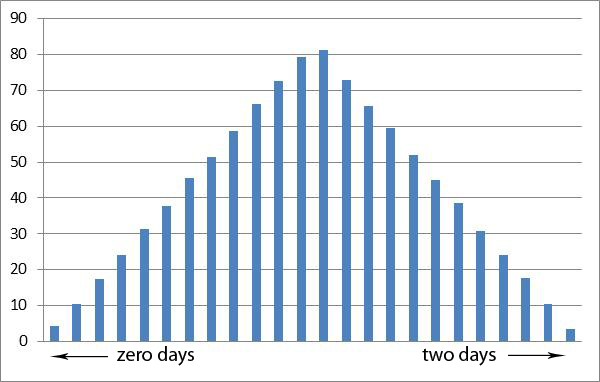
\includegraphics[width=0.75\columnwidth]{ChapterABM/figures/PermuteGapHistogramPSD}%
\caption{Histogram: ten thousand agents over a thousand days, 24 bins, showing how many times on average agents have an action gap between zero and two days, when the order of actions is permuted randomly on each turn.}%
\label{fig:permuteGap}%
\end{figure}

The model uses a single static `Randoms' class to provide consistent randomisation globally. A random seed provides both exact repeatability and the ability to change the seed for model runs where aggregate results require a full random spread of outcomes.

Randomisation of agents' timing can be used to avoid artifacts arising as a result of agent order (\citealt{gilbert_agent-based_2007} pp.27) but it raises its own problems. Consider a common scenario where the order of all agents' decision points are randomly permuted on each iteration. The probability of getting any particular point in that order is the same for all agents. However, over \emph{two} days, the time between any one agents' actions will vary. The most common outcome is an exact one day gap, since it has the highest possible number of chances to appear from both days' permutation: a one-day gap can fit into a two-day space beginning at any point on the first day, right up to the last slot. If $n$ is the number of agents being permuted, there are the same number of one-day gaps as $n$. Each consecutive length of shorter gap has $n-1$ chances, until at both extremes (with a small but equal probability), two actions will either be consecutive (at the very end of one day and the beginning of another) or nearly two full days apart. The result is a pyramidal distribution. The histogram in figure \ref{fig:permuteGap} confirms this from a model run for actions of ten thousand agents with daily randomly permuted actions, over a thousand days.


Using a random permutation, then, the time between actions will never be consistent. However, over many iterations, this averages out, so why should this be a problem? It is important to be aware that the above dynamic exists, as it can explain errors in agent decisions that would otherwise remain mysterious. Any decision process based on feedback between $t$ and $t+1$ may be affected. One of these situations is this: a scenario with both Firms and People, where Firms make decisions based on responding to a change in net income between iterations. Any Firm presuming the gap to be a full day will be using faulty data. There are (at least) three ways around this. Firstly, the actions of People and Firms can be put into two `bins' and permuted separately. This guarantees that all People will have made their decisions before Firms come to act. Second, Firms can be allowed to know the length of time between decision points and alter their decision-making (for example, by correcting the rate of change of net income accordingly.) Third, some other method of permuting that damps the variability between timesteps could be used, such as a random walk. This thesis uses the first of these. 

\subsection{Economies of scale and avoiding the need for strategy \label{sec:abmprod}}

As section \ref{sec:prodfuncts} discussed, considered statically, \gls{eos} are entirely straightforward: an equation describes the relationship between the level of input and the given output. But if many agents are deciding whether to input time into a production function, how do they decide? The best choice will in part depend on the levels of output available from Firms – but this is determined by what all other agents have decided. This leads to a catch-22: should an agent wait to see what others do? If everyone does this, how can production get going at all? Once they have made a decision, how is the output itself determined – or more specifically, when, given that both input and output are flows in a multi-timestep situation?

If agents are deciding simultaneously, this can be framed as a game-theoretic problem, solveable for small numbers of agents, but increasingly problematic with larger numbers, and impossible if agents are not synchronised. The choice agents must make in this situation shares something of the dynamic in the ``El Farol Bar problem'' (\citealt{ arthur_inductive_1994}). Everyone makes a decision about going to the bar, but if more than a certain percentage turn up, it is so crowded that no-one is happy. All agents, however, must decide simultaneously. Edmonds describes it thus:

\begin{quote}
``Any model of the problem that is shared by most of the agents is self-defeating. For if most agents predict that the bar will not be too crowded then they will all go and it will be too crowded, and vice versa.'' (\citealt{brenner_modelling_1999} p.12)
\end{quote}

The \gls{eos} problem is the same dynamic in reverse: all agents gathering in one Firm will give a \emph{higher} payoff, but there is no way to know who will choose where. The thesis model uses a `granular' approach to avoid these pitfalls. While it has its own issues, it does manage to successfully power the `transmission belt' between production and welfare. This method will be described first, followed by a more detailed discussion of its rationale. The following section (\ref{sec:blindvsrational}) also discusses a more detailed `pseudo-code' thought experiment examining the catch-22 problem.

In the thesis model, when agents decide where to contribute their input, they do so then and there, at the point of decision. They then \emph{leave} their input with whoever received it until their next turn to act. It stays there for one whole `day' (on average, given randomisation of agent order, see section \ref{sec:randomisation}), when it is removed by the same agent prior to re-taking the decision. At the same time, the quantity of output produced is \emph{also} worked out. This is done from the producers rolling record of the quantity of contributed input from all agents. Let the producer's total current contributed input be $T_p$. When an agent adds their input, $t_a$, this rolling record can be used to calculate the output from the agent's contribution, $g_a$:

\begin{equation}
g_a = f(T_p) \cdot (t_a / T_p)
\end{equation}

Here, $f(T_p)$ is the \gls{eos} function, giving a total output figure from all current input. The agent's input divided by the total input, $t_a/T_p$, gives the proportional contribution of that agent. These two can then be multiplied to give $g_a$, the `granular' quantity of extra output produced at that point, which goes into the producer's stock.

What are the problems with this approach? Simply that agents are forced to make optimising decisions given static information: they are robbed of the ability to even attempt to make strategic decisions or develop expectations. Given what has just been said, however, it is the structure of the problem itself that robs them of strategy. The issue here, as Oeffner points out, is the difference between risk and `true uncertainty' (\citealt{oeffner_agent-based_2008} p.25-6). The problems described above represent true uncertainty: probabilistic outcomes are incalculable. As Oeffner points out, agents with `rational expectations' in these situations will do no better than myopic ones. 

Exactly the same issue arises for space-cost decisions in the presence of density costs in section \ref{sec:results}, though the model in section \ref{sec:firmsLoV} looks at a situation where risk is a component. (The ideas in that model are discussed below in section \ref{sec:dmr}.)

%Bits:
%It occurred to me looking at the Excel sheet, I don't actually have the output from each Firm - which is just currentContributedTime input into the production function. That's what the flow is; it's kind of equivalent to "watts". So it's the rate of production. People add and remove themselves from this rate between decision points; it's not really a `trick', it kind of makes sense.
%Comments nabbed from connected models chapter:
%Where have I mentioned the curve and magnitude parameters for smooth EoS? Also point out that the smooth EoS allows separate control of inc rets and linear parts in model, which is helpful. Wouldn't be in analytic version, it'd make it messier. Whole point there is it enables algebraic simplifications / normalisations.
%Wherever I do this, make this point: useful simplifications for the transmission belt model are different to those for the CM. They work better here. It turns out, having worked with the simple maths a little. So again, "everything depends on the problem" continues to be the most useful five words ever.
\subsection{Blind versus rational choice: an illustration of the problem with economies of scale \label{sec:blindvsrational}}

This section looks at a small concrete example of the interdependency of decision structures and model `world'. The \gls{coremodel}-style of \gls{increts} \eqref{eq:coremodelMprod} is used, with the fixed labour requirement set to 3. This means that no production is possible at all unless three units of labour are input: an indivisibility. This is straightforward enough to impose analytically, but how might it work in an agent context? 

Consider a scenario where agents choose an employer and goods in the same `moment' (that is, during one action). Assuming that they are completely myopic, zero-intelligence agents, they are unable to make judgements about future timesteps. As a result, they will not work if no goods are available. There is no point: there is nothing to buy. Equally, if no work is available, they cannot \emph{afford} to buy anything. This can lead to a catch-22: if Firms have no stock, they need labour to make more, but no-one will work if no stock is available. Compare these two possibile approaches agents might take in this situation, both of which have arisen as solutions for getting agents trading:

\begin{enumerate}
	\item A `rational choice': agents decide sequentially, looking at what Firms are producing in order to choose whether to work. If no goods are available to buy, there is no point in working.
	\item A `blind choice': At $t$, agents randomly choose a potential employer. If at $t+1$ this was successful, they repeat the same action. 
\end{enumerate}

The first of these, `rational choice', assumes agents are able to rationally choose a workplace. However, each agent is only able to contribute one unit of labour; a Firm needs three to even begin producing. Less than three, and output is zero. The second, `blind choice', is not completely blind, since the search requires agents to have the most fundamental attribute required for rationality: to be able to tell on the next turn whether their guess made them better or worse off. 

The `rational choice' result is that no work takes place and nothing is produced: production cannot get started because each single agent considering their options can never get above contributing one unit of time.  The blind choice, however, does stand a chance of success. Actors select a random Firm to work for, and see if it improved things on the next day. If it did, they can stick with the same strategy. In the example of a fixed labour requirement of three, even with a set of agents consisting of only four People and $n$ Firms, given enough time they would all randomly find themselves selecting the same Firm and allowing production to take place.

The smooth production function \eqref{eq:smoothEoS}, while lacking a tidy definition for fixed and marginal labour, works in both `blind' and `rational' cases, since any amount of labour will always produce some quantity of output. It is this function that the thesis model uses, since it– again – offers a route for avoiding some of the complexities inherent in the model's interdependencies. Section \ref{sec:examplesmapping} discusses this choice further.


\subsection{`Data, meaning, response' \label{sec:dmr}}


A final manifestation of uncertainty for Actors comes from the feedback process of \gls{dmr}. This idea is taken from Jane Jacobs' final book, `the Nature of Economies' (\citealt{jacobs_nature_2001}). In it, Jacobs looks for the common thread that ties supply and demand to other feedback mechanisms in nature. She settles on the importance of integration between `the data, the meaning of the data and appropriate responses to the data.' (p.109) That framework functions, she argues, for systems as disparate as a termite mound, where supply and demand of soldier termites is precisely controlled through distributed pheromone signals, and price data, which can ``carry meaningful information on imbalances of supply and demand and automatically trigger corrective responses'' (ibid p.110). 
%That tripartite split - data, meaning of the data, appropriate responses to the data - is very useful for thinking about how to develop agent-based models of economic activity.

Cybernetician Stafford Beer cites weather vanes as exemplars of perfect `intrinsic control': ``it is the wind that is capricious; the measurement does not make mistakes.'' (\citealt{beer_what_2002} p.214) In this case, \gls{dmr} collapses into a single instantaneous feedback. As he points out, ``a great deal depends on the speed of the response'' (ibid). In situations with slower responses, meaning links data to response – and this opens up the possibility that an Actors' interpretation may lead to \emph{in}appropriate responses. An incorrect meaning assigned to data could come from several sources. One of these – not used in this thesis – is simply that the data may be context-specific. Spedding has an example from cattle markets that illustrates this point nicely: 
%This fact alone helps explain why the `granular' approach to stock-pricing produces a functioning model in section \ref{sec:prodtowelfare}.  

\begin{quote}
``Even when good information is ostensibly available, it may not be precise enough. For example, published statistics would suggest that there is a fortune to be made by transporting top-quality Friesian calves from one market in East Anglia to another no more than twenty or thirty miles away. This is not, in fact, the case - it simply happens to be the practice to sell them rather older and heavier in one market than in the other, and in consequence they fetch a somewhat higher price there.'' (\citealt{spedding_freams_1983} p.458)
\end{quote}

In this case, the agents actually need metadata to help formulate its meaning. But even when all agents share a common metadata understanding, as is the case in the thesis model, meaning can be misinterpreted. The model in section \ref{sec:firmsLoV} looks at an example that boils Actors' decision process down to make the \gls{dmr} dynamic as clear as possible. Firms move and then decide if that action was appropriate based on one datum - revenue change. The simplest interpretation of the data - Firms' take on its meaning - is, `did my revenue increase? Then the action was a success.' 

\gls{dmr} is a kind of informational `sonar'; as Vives puts it, firms often ``use prices to experiment and learn about demand or costs conditions. Experimentation consists of paying a short-term cost in order to gain information that yields a long-term benefit'' (\citealt{vives_oligopoly_2001} p.291). This is a very important component of respecting the impositions of space on the market, discussed in chapter \ref{chapter:ABM}, where agents must collect information however they can.

Much of the model finds ways to avoid this sort of coordination problem. The \gls{abm} tendency toward descriptive mapping makes this sort of problem very prominent: as section \ref{sec:decstruct} discussed, if autonomous agent-building is the central goal, \gls{dmr}-like issues will arise. One of the key aims of the `mobile Firm' models in section \ref{sec:mobFirms} is to investigate what a large hurdle to full coordination \gls{dmr} can be.

%DMR straddles the line between \gls{oop} encapsulation and dependencies, explicit code and implicit structure and meaning. The `M' in \gls{dmr} does not have to exist in explicit code form; it is up to the modeller to think through where it is, what it is and what the best approach to coding it is.

\subsection{Examples of descriptive versus functional mapping \label{sec:examplesmapping}}

This chapter ends with some examples of how the difference between descriptive and functional mapping (section \ref{sec:code_vs_function}) shows itself in the thesis model. The most obvious example is that a single class takes care of utility (see section \ref{sec:howPeopleAct} for full details). Each Person asks this centralised class what utility they can get from a given bundle of goods. In reality, of course, the process of deciding what to buy takes place in a person's head: they do not ask some centralised organisation to tell them what they like. While it would be entirely possible to give each Person agent their own private methods for working out their wants (a closer descriptive mapping), in this case there is nothing to be lost by having a single class do the job.  Of course, this does not rule out situations where it may be advantageous to internalise these decisions to each Person, as well as good computational reasons. If, for instance, agents were running on several parallel threads, having to calculate utility through a global class would slow the model down.

The method of modelling production used in the thesis is not convincing as a model of actual production and is not meant to be. It attempts to solve much the same issue the \gls{coremodel} does: how to link production to welfare via demand? The difference is in requiring disaggregated agents to achieve this. The choice of a smooth over \gls{coremodel}-style \gls{eos} function is, in this light, based on what achieves that goal, rather than on which manages to be `more realistic'. 

The same applies to the model's prevalent use of the \gls{ces} function. Fujita \emph{et al.} suggested a subtitle for their work might be ``games you can play with CES functions'' (\citealt{fujita_spatial_2001} p.6), and the same applies here: it is a swiss-army knife of a function, but as with \gls{eos}, it stands in as a proxy for much more involved processes. For instance, in the thesis models a single Actor can buy any number of goods, each with a separate location and price. No uncertainty is involved in the spatial or price search, no actual travel or coordination issues arise. Equally, the \gls{ces} can be used to avoid \gls{bertcomp} dynamics where the Firm offering the highest wage (however marginal the difference) gets all the labour. Any more complex, `realistic' model of actual job markets, able to account for the fact that Bertrand dynamics do not in fact exist in the labour market, may be overkill. A \gls{ces} approach is used in the model in section \ref{sec:prodtowelfare}. This is, for the purposes of the model, very useful: functionally mapping the idea of how good cost may affect Actors' acquisition while avoiding detailed dynamic problems. This in no way lessens the importance of understanding those dynamics, of course.

\subsubsection{Number of Actors \label{sec:agentnumbers}}

\begin{quote}
Nigel Tufnel: What we do is, if we need that extra push over the cliff, you know what we do?

Marty DiBergi: Put it up to eleven.

Nigel Tufnel: Eleven. Exactly. One louder.

Marty DiBergi: Why don't you just make ten be the top number and make that a little louder?

Nigel Tufnel: [pause] These go to eleven.
\end{quote}
\hspace*{10cm}\emph{\citealt{reiner_this_1984}}
\vspace{1cm}

In \gls{abm}, agent number is commonly afflicted by descriptive mapping. Each model agent is asked to represent a specific real-world counterpart, and the impact of agent number on outcome is taken to be always relevant. If for computational reasons too few agents can be created, aggregate stand-ins may be used. Approaches include aggregating agents into `super-individuals' or using a `technical fix' such as parallelisation and higher processing power (\citealt{parry_comparative_2008}) or combining an agent element with another aggregate modelling approach like gravity models to create a `hybrid' (\citealt{heppenstall_hybrid_2005}). In a recent example, an Economist article argues for an agent modelling of `the entire economy' involving `millions of agents' (\citealt{economist_new_2013}). The first thing to consider, however, is what the purpose of agent number is in any particular model.

Many economic arguments analyse away any effects from agent number; as section \ref{sec:marketstructure} outlined, this is how market structure problems are often circumvented. For example, the assumption of price-taking in perfect competition models requires an unspecified `large' number of agents, so that no single one can influence price. As Blaug says, ``perfect competition is, of course, an oxymoron, since it is a case of no competition whatsoever between firms'' (\citealt{blaug_trade-off_2009} p.223).

Within \gls{abm} there is an implicit assumption that such effects should be accounted for. After all, isn't that the very reason for disaggregating the model in the first place? The answer is, it depends. Just because a number of agents are being used does not mean every number-related effect should be considered. There may be good reasons for excluding them. Most obviously, the modeller may want to ignore some small number effect without having to actually increase agent numbers to do it, simply because of the computational expense. Functional-mapping-wise, this leads to a counter-intuitive point: it is possible to say `assuming large numbers' while only having a small number of agents, if the dynamic under examination is separate from the assumption. For instance, the modeller may want to assume fixed prices as in perfect competition. This could be justified by assuming that numbers exogenous to the model are large, implying the model is only one region in a much larger world where, for example, fuel prices are set exogenously. But equally, if the goal is to have a number large enough to produce reliable aggregate results (e.g. which regions get what proportion of agents?), it may be just as unnecessary to force a large enough number to avoid sub-perfect-competition dynamics. The price-taking assumption could still hold without invalidating the choice of number.

A related aspect of number is that, for many of the partial models presented in the next chapter, no interaction is taking place between agents. Using partial models is the easiest way to avoid the problems imposed by full coordination. Depending on the problem, any number of model features and variables can be fixed. This is also a very effective method for testing and is used extensively in chapter \ref{chapter:models} to do so. 

The `partial' models presented here fix different quantities depending on the problem. Most often, all People get a fixed wage (or a wage determined by the model); this means the overall level of demand is set exogenously. Firms' stock levels do not change: stock is always available to meet demand. All Firms have to do then, is maximise revenue by attempting to capture as much demand as they can. Aside from these two key features, others do vary. Firms may be mobile, optimising their location, while People remain immobile, and vice versa. In partial models using the \gls{ces} function, the number of Firms – each providing a unique good – will affect the total possible quantity of utility. 

Where People are deciding on location, if wages and prices are fixed, stock is unlimited and no density costs are incurred, each makes decisions entirely independently of the others. As a result, there is no actual difference between running a model with one agent a hundred times, or a hundred agents once (i.e. they are ergodic). There is, however, a reason for running a multi-actor model in this situation: it allows for a quick understanding of the outcome of the underlying stochastic process. Outcomes can be similar to entropy models (\citealt{wilson_entropy_1970}) or can produce `indifference maps' showing the spread of agent location choices.

In situations where there is interaction, agent number may matter for reasons unique to the problem being modelled. The \gls{dmr} model in section \ref{sec:firmsLoV} discusses a number of ways agent number interacts with noise levels. Finally, the `transmission belt' model in section \ref{sec:prodtowelfare} has its ability to swiftly find equilibrium affected by total agent number.
%Section \ref{sec:spatvsnon} shows the specific affect that Actor number can have when density cost and a hard space cost limit interact: agent number can increase to the point where utility levels above zero become impossible because of density costs.

Agent number, for the thesis model framework, has a somewhat prosaic purpose: to help with its functioning as an `experiment station', numbers are chosen to allow a balance between good interaction speed and good presentation while also allowing for effectively robust emergent properties. 

\section{Summary}

This chapter has detailed the way the thesis model has been put together. It has also discussed the broader issues that arose as a part of the logical journey of model development, and described some ways in which a `functional mapping' has taken precedence over a `descriptive mapping'. The next two chapters present results from this framework.

